\section{Density matrix of two energy level system}

\begin{figure}[h!]
	\centering
	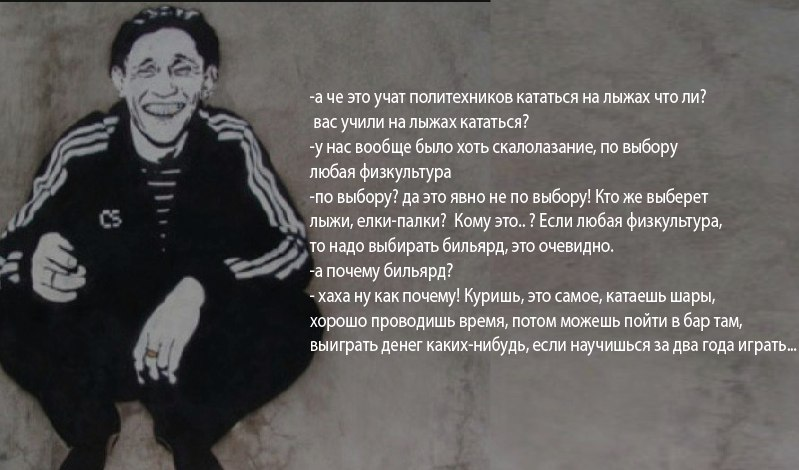
\includegraphics[width=0.8\linewidth]{fig/L4/true_Baiko}
	\caption{The true essence of life choices}
	\label{fig:truebaiko}
\end{figure}

Let consider a two-level system again. In section \ref{sec:atom-field_interaction} we obtained Rabi osculations. Needless to say there weren't any dissipative forces, so turning off the incident field will make the system <<freeze>> in the last state forever (fig. \ref{fig:turnofffield}). It is obvious that it is not happening in actual truth due to an interaction with immediate media. Adding phenomenological terms to equations for $C_a$ and $C_b$ (e.g. \eqref{eq:rabi_system}) is incorrect because we don't know time dependence of $\ket{\psi(t)}$. The correct way is to use \textit{density matrix formalism}.

\begin{figure}[h!]
	\centering
	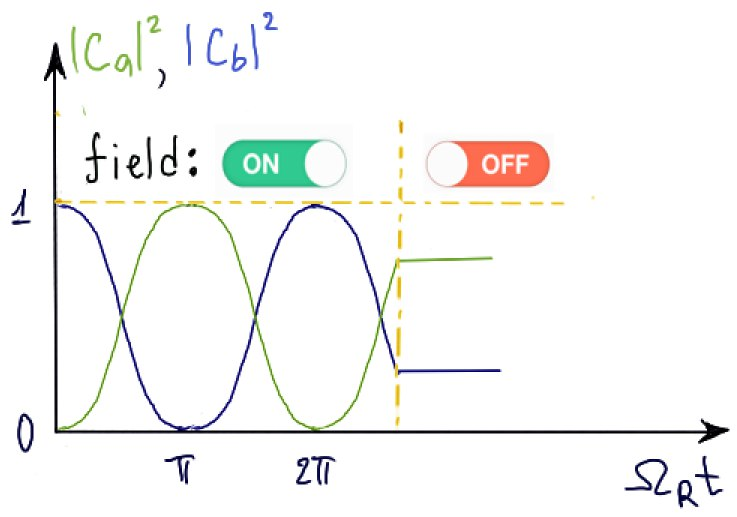
\includegraphics[width=0.5\linewidth]{fig/L5/turn_off_field}
	\caption{Turning the incident field off}
	\label{fig:turnofffield}
\end{figure}


A density matrix is a matrix that describes a quantum system in a mixed state, a statistical ensemble of several quantum states. In other words, density matrix is very useful if we do not know a wave function which contains all the information of the system but we still want to describe our system. There are two possible options (fig. \ref{fig:densmatr}):
\begin{enumerate}
	\item $\ket{\psi_A}$ is known but we need to describe only $B$-system which is intersystem of $A$-system.
	\item $B$ --- is not a conservative system and energy exchanging with reservoir is taking place.
\end{enumerate}
\begin{figure}
	\centering
	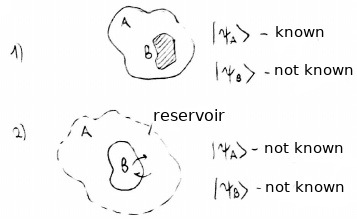
\includegraphics[width=0.7\linewidth]{fig/L5/dens_matr}
	\caption{Possible systems where one need to use density matrix}
	\label{fig:densmatr}
\end{figure}
If $\ket{\psi}$ is known than density matrix is defined by
\begin{equation}
	\boxed{\hat{\rho} = \ket{\psi} \bra{\psi}}
\end{equation}
If we expand to Fock states $\ket{\psi} = \sum C_n \ket{n}$ then 
\begin{equation}
	\hat{\rho} = \sum_{nm} C_n^* C_m \ket{m} \bra{n}.
\end{equation}
Matrix elements --- $\rho_{nm} = C_n^* C_m$.

\begin{testexample}[Density matrix for two-level system.]
	%\textcolor{red}{(UNCOMMENT THIS LATER! (see source))}
	For two-level system we have:
	\begin{equation}
		\ket{\psi} = C_a \ket{a} + C_b \ket{b},
	\end{equation}
	so
	\begin{equation}
		\hat{\rho} = \ket{\psi} \bra{\psi} = 
		\begin{pmatrix}
			\left| C_a (t) \right|^2 & C_a (t) C_b^*(t) \\
			C_b (t) C_a^*(t) & \left| C_b (t) \right|^2
		\end{pmatrix}, \qquad
		\rho_{ij} = \bra{i} \hat{\rho} \ket{j}.
	\end{equation}
\end{testexample}

Mean operator value:
\begin{equation}
	\bar{f} = \bra{\psi} \hat{f} \ket{\psi} \sum_{nm} C_n^* C_m \bra{n} \hat{f} \ket{m} = \sum_{mn} \rho_{nm} f_{nm} = \Tr \left(\hat{\rho} \hat{f}\right).
\end{equation}
\textit{This is the main intended use of density matrix!} Properties:
\begin{enumerate}
	\item Hermiticity: $\hat{\rho}^{\dagger} = \hat{\rho}$.
	\item $\Tr \hat{\rho} = 1 \quad \to \quad$ diagonal elements: $\rho_{mn} = \left| C_n \right|^2$.  Remark: only for pure states!
	\item $]\  \hat{\rho} = \ket{\psi} \bra{\psi} \quad \to \quad \hat{\rho}^2 = \hat{\rho}$. It's easy to show:
	\begin{equation}
		\hat{\rho}^2 = \ket{\psi} \underbrace{\bra{\psi} \ket{\psi}}_{\hookrightarrow = 1} \bra{\psi} = \ket{\psi} \bra{\psi}.
	\end{equation}
	It also means that density matrix of pure state --- projector.
\end{enumerate}

\subsection{Density matrix of mixed state}

Now let us consider a \textit{mixed state}. Let there are lots of systems in different pure states $\ket{\psi_i}$. Let there are $N_i$ particles in $\ket{\psi_i}$, then the whole amount of particles (=systems) is $N = \sum N_i$. The probabily to find any system in $\ket{\psi_i}$ is $\omega_i = \frac{N_i}{N}$. The question we are trying to answer now: how can we find mean operator value?
\begin{equation}
	\bar{f} = \Tr \hat{\rho} \hat{f} = ? \qquad \text{since} \quad \hat{\rho} = ? 
\end{equation}
Scenario is the following:
\begin{enumerate}
	\item Calculation of quantum-average values: $f_i = \bra{\psi_i} \hat{f} \ket{\psi_i}$.
	\item Calculation of classical average values: $\bar{f} = \sum \omega_i f_i$.
\end{enumerate}
So
\begin{multline}
	\bar{f} = \sum \omega_i \bra{\psi_i} \hat{f} \ket{\psi_i} = \sum_i \omega_i \sum_{nm} \underbrace{\left( C_n^i \right)^* C_m}_{\rho_{mn}^i} \underbrace{\bra{n} \hat{f} \ket{m}}_{f_{nm}} = \\
	= \sum_{nm} \sum_i \rho_{mn}^i \omega_i f_{nm} \myeq \Tr \left( \hat{\rho} \hat{f} \right).
\end{multline}
Here we defined density matrix as $\left( \hat{\rho}_{\text{mix}} \right)_{mn} = \sum_i \omega_i \rho_{mn}^i$. Density matrix has a probability meaning:
\begin{equation}
	\hat{\rho}_{\text{mix}} = \sum_i \omega_i \hat{\rho}_i, \qquad \hat{\rho}_i = \ket{\psi_i} \bra{\psi_i}.
\end{equation}
Coefficients $\omega_i$ are defined by \textit{statistical (not quantum!) mechanics} (e.g. Boltzmann distribution).

Remarks:
\begin{enumerate}
	\item $\Tr \hat{\rho}_{\text{mix}} = 1$ by virtue of the fact that $\sum \omega_i = 1$.
	\item $\Tr \hat{\rho}_{\text{mix}}^2 = \sum \omega_i^2 \le 1$. 
	
	Proof:
	\begin{multline}
		\Tr \hat{\rho}_{\text{mix}}^2 = 
	\end{multline}
	It means it is not projector anymore! Testing criterion of pureness is introduced by
	\begin{equation}
		\boxed{\mu = \Tr \hat{\rho} - \Tr \hat{\rho}^2 \ge 0}
	\end{equation}
\end{enumerate}

\subsection{Subsystem density matrix}